
学习线程安全的数据结构之前,必须知道需要哪些数据结构。如果这是一个简单的问题——多个线程可以同时使用的数据结构——那么你还太天真了。开始设计并发程序中使用的新数据结构或算法时,就知道这个问题有多么重要了,以至于怎么强调都不为过。这句话应该让你感到警惕,并停下来思考。实际情况是,线程安全的数据结构没有一个明确定义适合每种需求和应用程序。

\subsubsubsection{7.2.1\hspace{0.2cm}线程安全的最佳方式}

可以从一些简单的,但在实践中容易遗忘的方式开始。高性能设计的一个原则是,\textit{不做总是比做要快}。当前,这个原则可以缩小为,对于数据结构是否需要线程安全?确保线程安全,意味着需要由计算机完成一些工作,我们真的需要吗?是否可以对计算进行调度,使每个线程都有自己的数据集进行操作?

在前一章中使用的线程安全计数器。如果所有线程始终看到计数器的当前值,这就是正确的解决方案。但当所需要的只是计算在多个线程上发生的事件,例如:分配给多个线程的一组大数据中搜索某些内容。线程在执行搜索时不需要知道计数的当前值。当然,需要知道计数的最新值来增加它,这是正确的,只有在所有线程上增加单个共享计数时才会出问题,就像这样:

\hspace*{\fill} \\ %插入空行
\noindent
\textbf{01a\_shared\_count.C}
\begin{lstlisting}[style=styleCXX]
std::atomic<unsigned long> count;
…
for ( … counting loop … ) { // On each thread
	… search …
	if (… found …)
	count.fetch_add(1, std::memory_order_relaxed));
}
\end{lstlisting}

计数的性能非常差,可以看到在基准测试中只做计数(不搜索):

%\hspace*{\fill} \\ %插入空行
\begin{center}
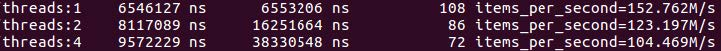
\includegraphics[width=0.9\textwidth]{content/2/chapter7/images/1.jpg}\\
图7.1 - 如果计数是共享的,对多个线程的计数不会修改
\end{center}

计数的改变实际上是负的,在两个线程上获得相同的计数要比在一个线程上花费更长的时间(尽管已经尽最大努力使用无等待的计数,同时使用最快的内存序)。当然,如果搜索比计数要长,那么计数的性能就无关紧要了(但搜索代码本身也可以在全局数据上做一些事,或者在每个线程的副本上做一些事,所以这是一个有指导意义的例子)。

假设只关心计算结束时的计数值,一个更好的解决方案是,在每个线程上保持本地计数,并且只增加共享计数一次:

\hspace*{\fill} \\ %插入空行
\noindent
\textbf{01b\_per\_thread\_count.C}
\begin{lstlisting}[style=styleCXX]
unsigned long count;
std::mutex M; // Guards count
…
// On each thread
unsigned long local_count = 0;
for ( … counting loop … ) {
	… search …
	if (… found …) ++local_count;
}
std::lock_guard<std::mutex> L(M);
count += local_count;
\end{lstlisting}

为了强调共享计数增量的不重要性,将使用互斥锁对其进行保护。通常,锁是更安全的选择,因为它更容易理解(因此,更难制造Bug),尽管在计数的情况下,原子整数会让代码更简单。

如果每个线程在到达结束之前多次增加本地计数,并且必须对共享计数进行增加的操作,那么这种变化几乎完美:

%\hspace*{\fill} \\ %插入空行
\begin{center}
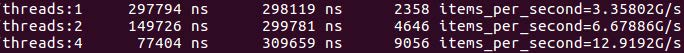
\includegraphics[width=0.9\textwidth]{content/2/chapter7/images/2.jpg}\\
图7.2 - 在多个线程上完美地计数
\end{center}

最好的线程安全是,不需要多个线程访问共享数据。通常,这种安排会以一些开销为代价,例如:每个线程维护一个容器或内存分配器,其大小会不断地改变。在程序结束之前不将内存释放给主分配程序,就可以避免锁定。代价是一个线程上未使用的内存不能提供给其他线程使用,因此总的内存使用将是所有线程峰值的总和(即使这些峰值使用时刻发生在不同的时间)。这是否可以接受取决于问题的细节和实现,这是每个开发者都必须考虑的问题。

当涉及到线程安全时,这个方案选择了逃避。从某种角度来看,确实如此,但在实际中经常出现这样的情况。在不需要共享数据结构的地方使用共享数据结构,并且性能提高非常明显,因此需要强调这一点。现在是时候来看看真正的线程安全了,其中数据结构必须在线程之间共享。

\subsubsubsection{7.2.2\hspace{0.2cm}真正的线程安全}

假设确实需要同时从多个线程访问特定的数据结构,现在就必须讨论线程安全了。但现在还是没足够的信息来确定线程安全意味着什么。前一章中讨论了强线程和弱线程安全保证。本章中,这样的分区已经不够了,所以这里不讨论一般的线程安全,而是应该描述数据结构提供并发访问的保证。

弱(但通常很容易提供)保证只要数据结构保持不变,多个线程就可以对相同的数据结构进行读取操作。显然,任意数量线程可以随时执行任何操作,并且数据结构保持在良好定义的状态,这种保证通常既昂贵又不必要。程序可能需要数据结构支持的某些(但不是所有)操作提供这样的保证。还有其他的简化版本,比如:限制访问数据结构的线程数量。

想要提供尽可能少的保证来保证程序是正确的,线程安全特性通常非常昂贵,甚至不使用时也会产生开销。

考虑到这一点,就可以开始研究具体的数据结构了,并看看如何提供不同级别的线程安全。

































